\vspace{3mm}
\textbf{Class prediction accuracy.} The aim of this experiment is to assess whether our models can correctly predict the class of the next event, given the time at which it occurs. For this purpose, we compare our models against Hawkes and RMTPP and evalute prediction accuracy on the test set.

\textit{Results.} We can see (Fig. \ref{fig:accuracy}) that our models consistently outperform the other methods on all datasets. Results of the other baselines can be found in Appendix \ref{detail-results}.


\begin{figure}
\centering
    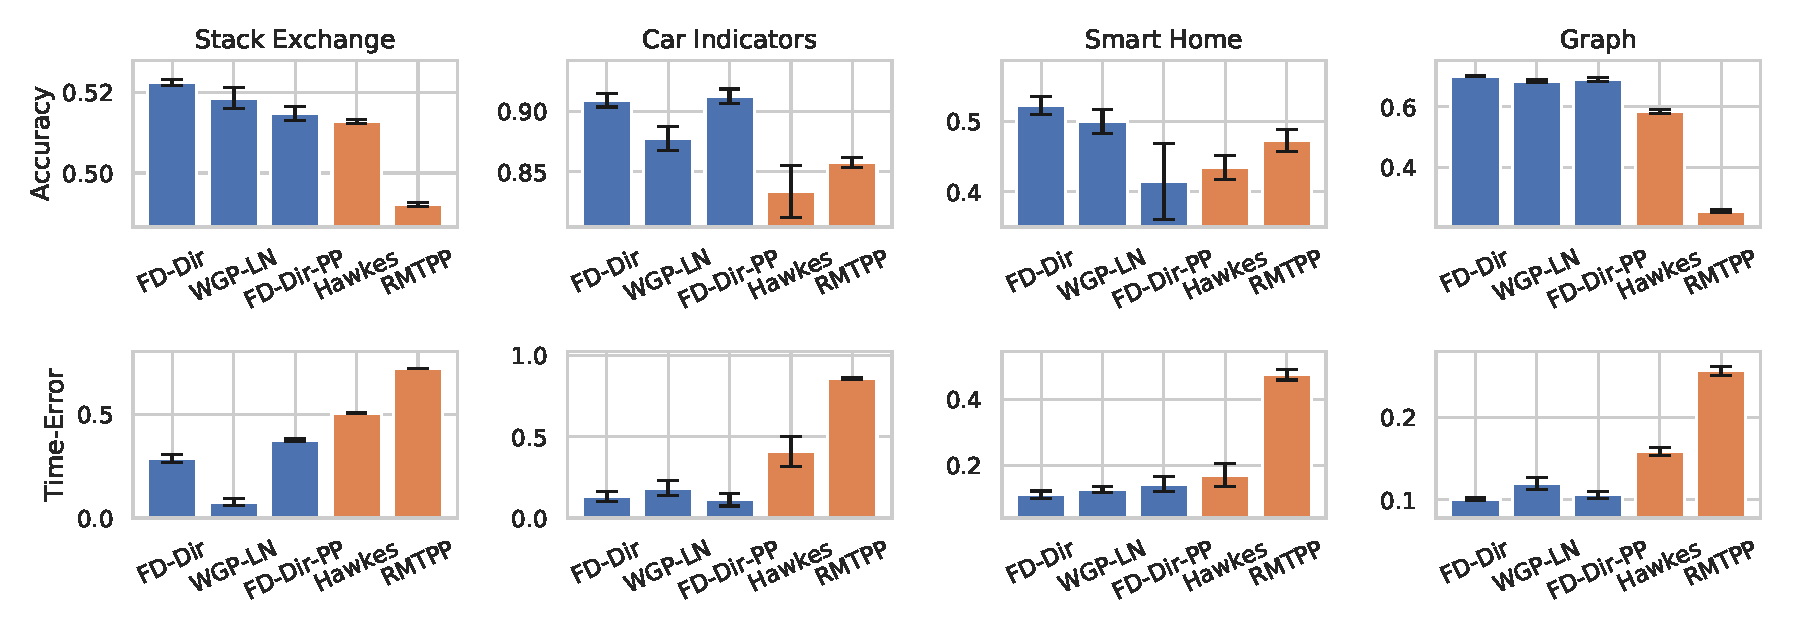
\includegraphics[width=\linewidth]{sections/010_neurips2019/paper/images/accuracy-final.pdf}
    \vspace*{-0.7cm}
    \caption{Class accuracy (top; higher is better) and \TimeScore (bottom; lower is better).}
    \label{fig:accuracy}
    \vspace*{-0.3cm}
\end{figure}
